\chapter{Проектирование предлагаемого решения}

\section{Внешнее проектирование}

\par
	В результате внешнего проектирования было получено техническое задание по ГОСТ 34.602-89 на разработку программного интерфейса (API) искомой системы, приведенное в приложении *.

\section{Внутреннее проектирование}

\par

	На основе требований, выдвинутых в техническом задании и результатов моделирования, приведённых в главе \ref{chap:models} проведено внутреннее проектирование API САТУ.

	Согласно требованиям, API САТУ взаимодействует с клиентскими приложениями через Интернет. В этой связи разумно использовать инструменты, ориентированные на работу в Web.

	Для разработки программного интерфейса системы анализа тепловых утечек в городских зданиях был выбран сценарный язык программирования PHP, поддерживающий концепцию ООП, поддерживающий концепцию объектно-ориентированного программирования. Основная причина выбора этого языка - распространённость его использования в web-проектах, в том числе для web-API, в силу наличия большого количества встроенных библиотек, ориентированных на разработку web-проектов.


\par

	Проектирование API выполнено на основе шаблона {MVC (Model-View-Controller)}, который подразумевает деление программного кода на 3 отдельных компонента: \textit{модель} (отвечает за обработку данных), \textit{представление} (отвечает за получение и отправление данных) и \textit{контроллер} (содержит управляющую логику, использует модели и представления). MVC позволяет сделать независимым код, отвечающий за работу с данными от кода, отвечающего за приём и отправку запросов [*].
	
	В качестве подхода к проектированию взаимодействия клиентских приложений и компонентов системы, работающих на сервере, была взят архитектурный стиль REST. Ограничения, определённые в REST, позволяют создавать масштабируемые и унифицированные программные интерфейсы [*]. REST использует в качестве протокола прикладного уровня HTTP.
	
	Стандарт, который использует API для форматирования сообщений - JSON. Формат JSON подходит для передачи сообщений со сложной структурой и уместен при обмене данными между клиентскими приложениями и сервером.
	
	Согласно требованиям в техническом задании (приложение \ref{app-tz}), а также алгоритму итогового оценивания энергоэффективности (раздел \ref{sec:models:algo:after}), API взаимодействует с данными САТУ с помощью СУБД, а именно обеспечивает загрузку и выгрузку снимков зданий. Таким образом, API необходим доступ к базе данных САТУ. Для инженерной реализации была спроектирована та часть базы данных САТУ, которая будет задействована в работе API. \\

	Проектирование базы данных выполнялось на основе ER-модели (“сущность-связь”). Соответствующая ER-диаграмма представлена на рисунке \ref{erd:1} и включает в себя основные сущности:

	\textbf{Пользователь} (\texttt{user}) - хранит идентификационные данные пользователей, их контакты, а также некоторые технические данные для системы аутентификации.

	\textbf{Здание} (\texttt{building}) - хранит данные из ГИС, необходимые для САТУ (в том числе результаты оценивания). Необходим для прикрепления к конкретным зданиям серий снимков.

	\textbf{Снимок} (\texttt{snapshot}) - хранит данные, полученные пользователями с различных устройств, в том числе ИК изображения (в двоичном представлении), координаты съёмки, а также данные, собранные со вспомогательных датчиков в момент съёмки здания устройством.

	\textbf{Серия снимков} (\texttt{snapshot\_series}) - используется для объединения снимков зданий, выполненных конкретным пользователем с помощью конкретного ИК устройства за определённый интервал времени. Это необходимо для правильного хранения версий снимков здания за счёт логических ограничений в структуре базы данных. 

	\textbf{ИК устройство} (\texttt{ir\_device}) - позволяет централизованно хранить всю техническую информацию об устройствах съёмки (тепловизорах). Таким образом, у клиентов нет необходимости отсылать эти данные после каждой серии съёмки.

	\textbf{Приложение} (\texttt{application}) - хранит идентификационные данные клиентских приложений, сведения об ограничениях доступа к функциям API и дополнительные сведения о его конфигурации.

	\textbf{Ключ доступа} (\texttt{token}) - предназначен для хранения ключей доступа, привязанных к приложению, а также информации об этих ключах: тип доступа(ограниченный/неограниченный), статус(активен/неактивен). Хранение токенов необходимо для того, чтобы исключить дублирование при генерации новых.

	\textbf{Журналы} (\texttt{log\_user}, \texttt{log\_application}) - используются для фиксирования некоторых действий пользователей и приложений в целях отладки клиентских программ.

	\pagebreak

	\begin{landscape}

		\begin{figure}[t!]
		      \centering
		      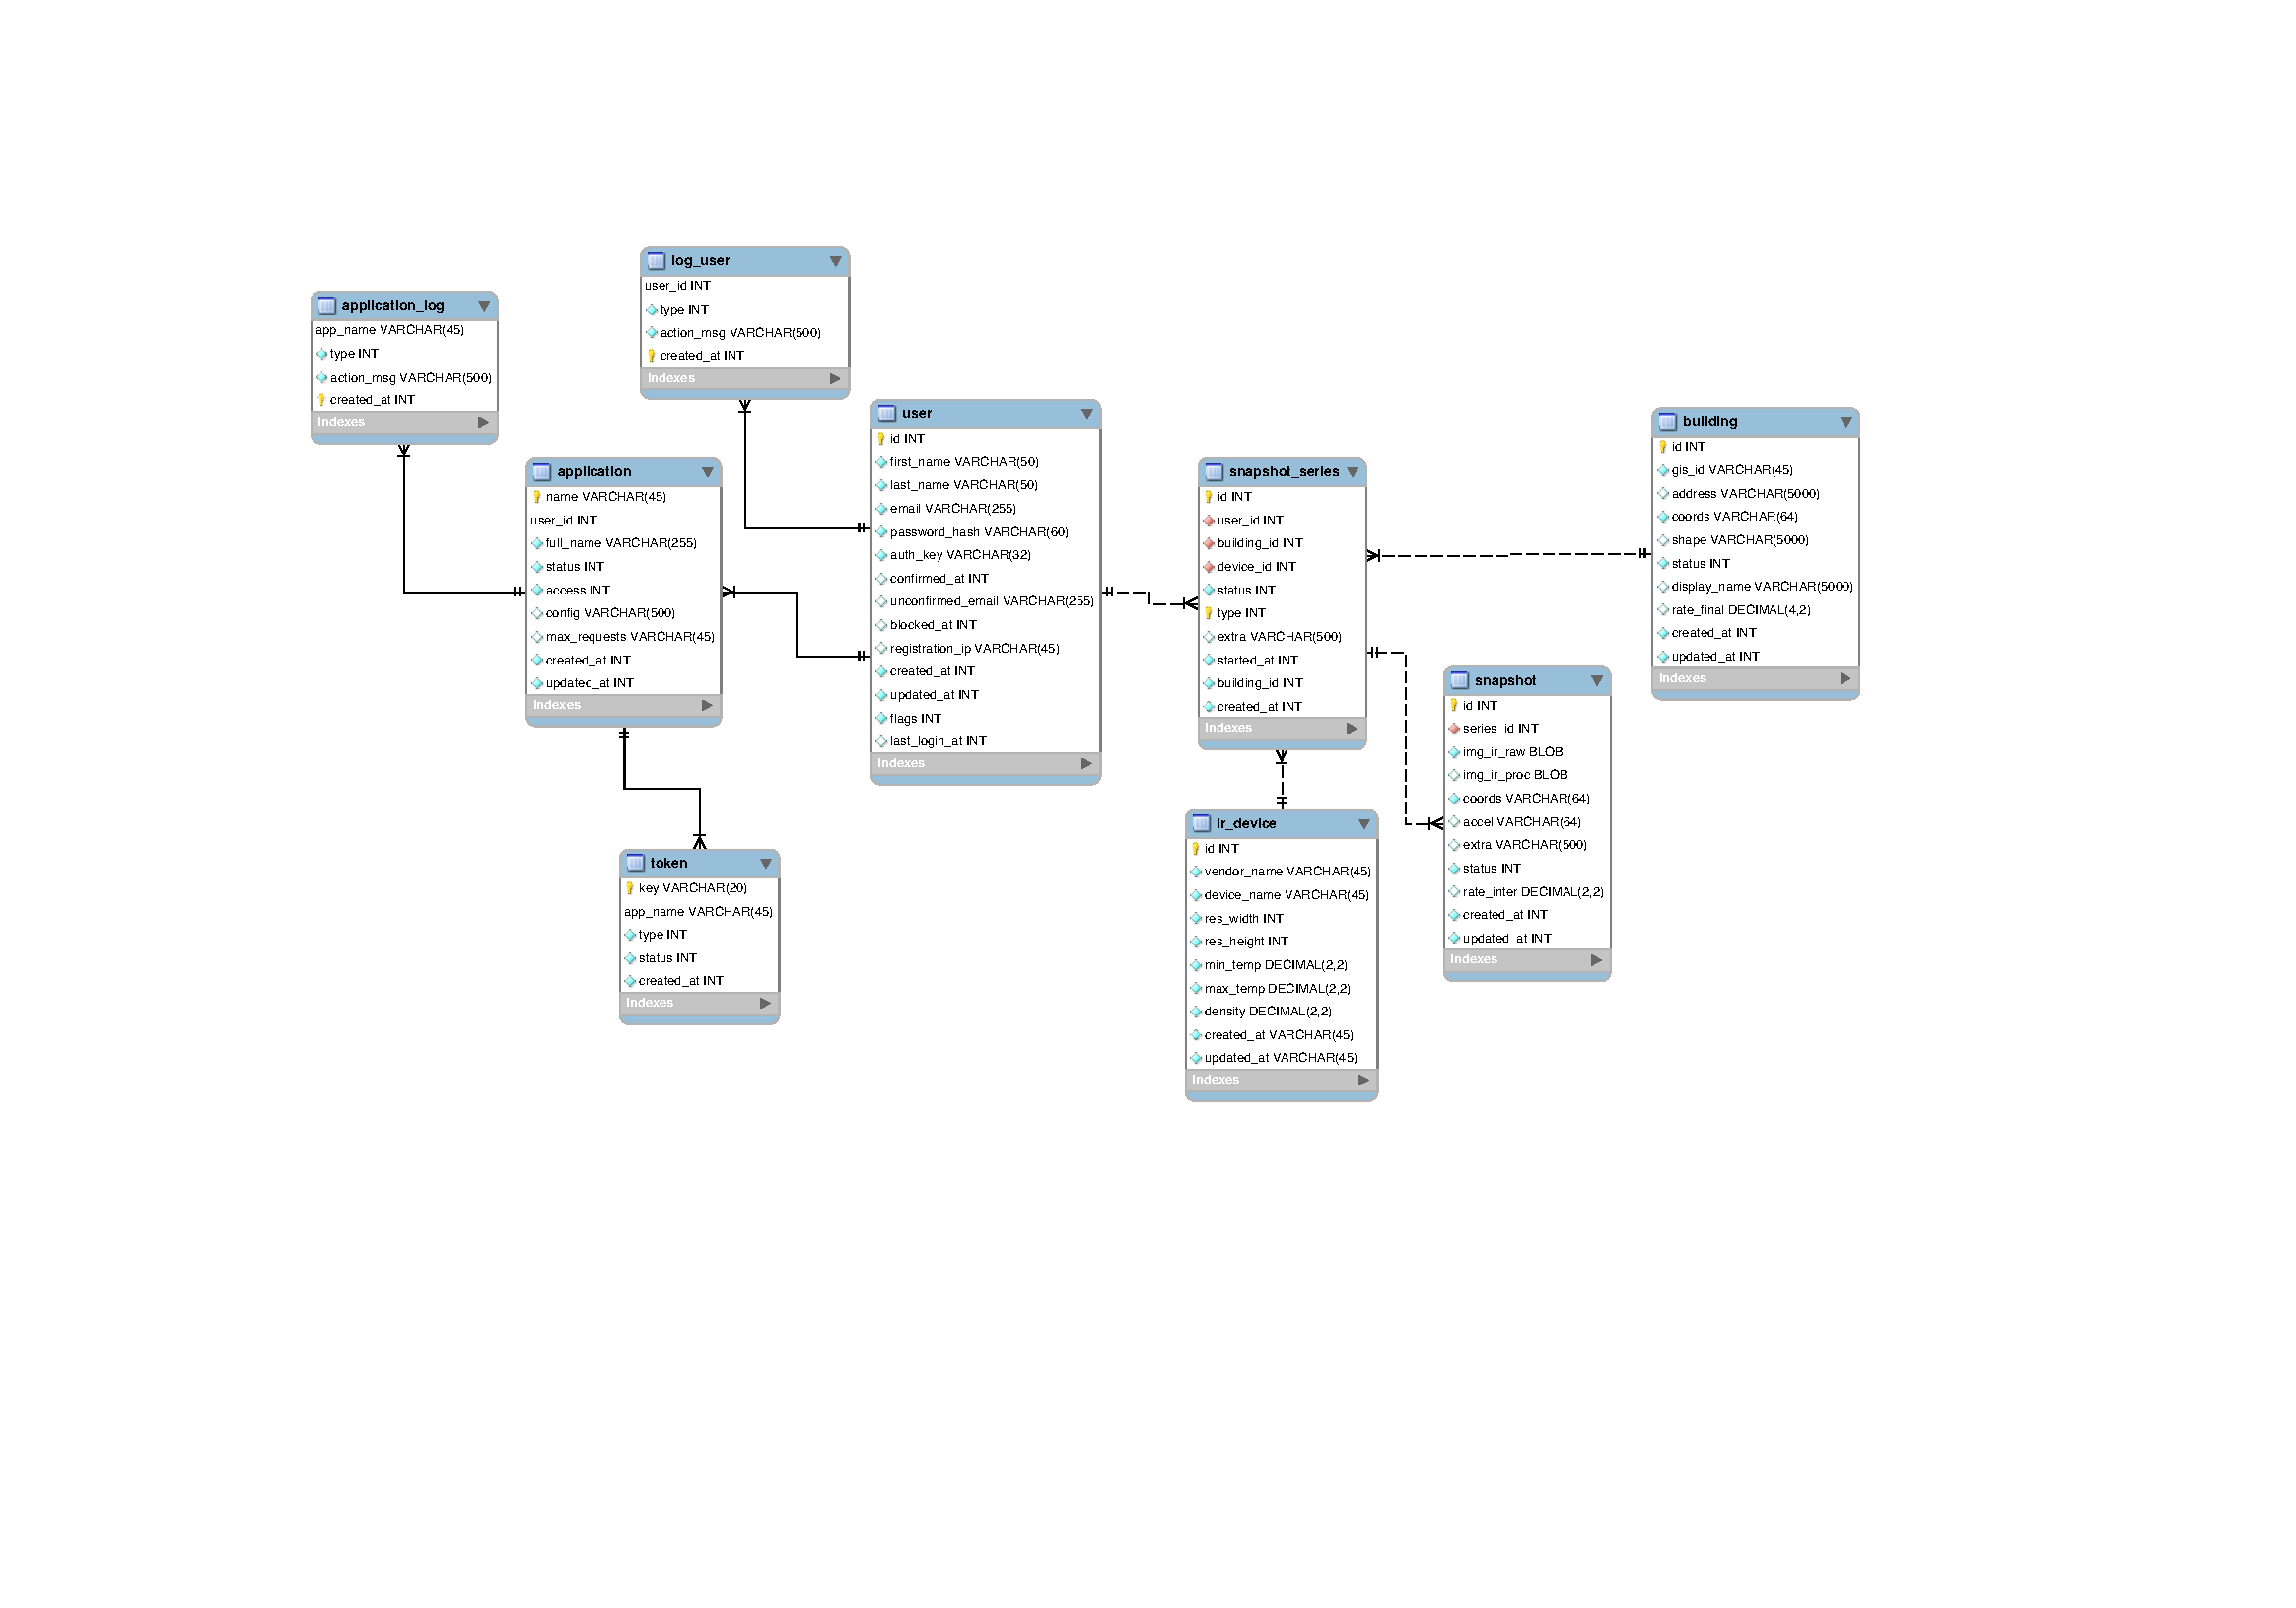
\includegraphics[width=1.3\textwidth]{images/erd/1}
		      \caption{Фрагмент схемы базы данных САТУ, используемой программным интерфейсом}
		      \label{erd:1}
		\end{figure}

	\end{landscape}

	\pagebreak

	На основе полученной схемы базы данных была спроектирована архитектура взаимодействия клиентских приложений с API путём изображения ресурсов, предоставляемых API и ссылок на эти ресурсы. Схемы, получаемые в результате проектирования, полезны при написании программного кода, когда точно сформулированы запросы, их параметры, определены необходимые для работы функций классы. Кроме того, эти схемы можно использовать при создании руководства программиста, поскольку в основном описывает набор доступных запросов, входные и выходные данные, их формат и структуру.

	При проектировании REST API используют диаграммы классов [ссылка]. Каждый ресурс характеризуется названием, идентификатором (URI), соответствующим HTTP-методом и набором параметров. Ресурсы на диаграмме изображены скругленными прямоугольниками. В качестве описателей входных и выходных данных ресурсов используют классы (выделены прямоугольной рамкой). Проектирование выполнено с помощью программного пакета Visual Paradigm 14.1, предусматривающего функцию генерации каркаса программного кода на основе построенных моделей.

	На рисунке \ref{uml:1} представлена диаграмма классов, описывающая набор ресурсов, специфичных для САТУ. Классы и ресурсы, относящиеся к авторизации пользователей и приложений, в данной диаграмме опущены.

	\pagebreak

	\begin{landscape}

		\begin{figure}[t!]
		      \centering
		      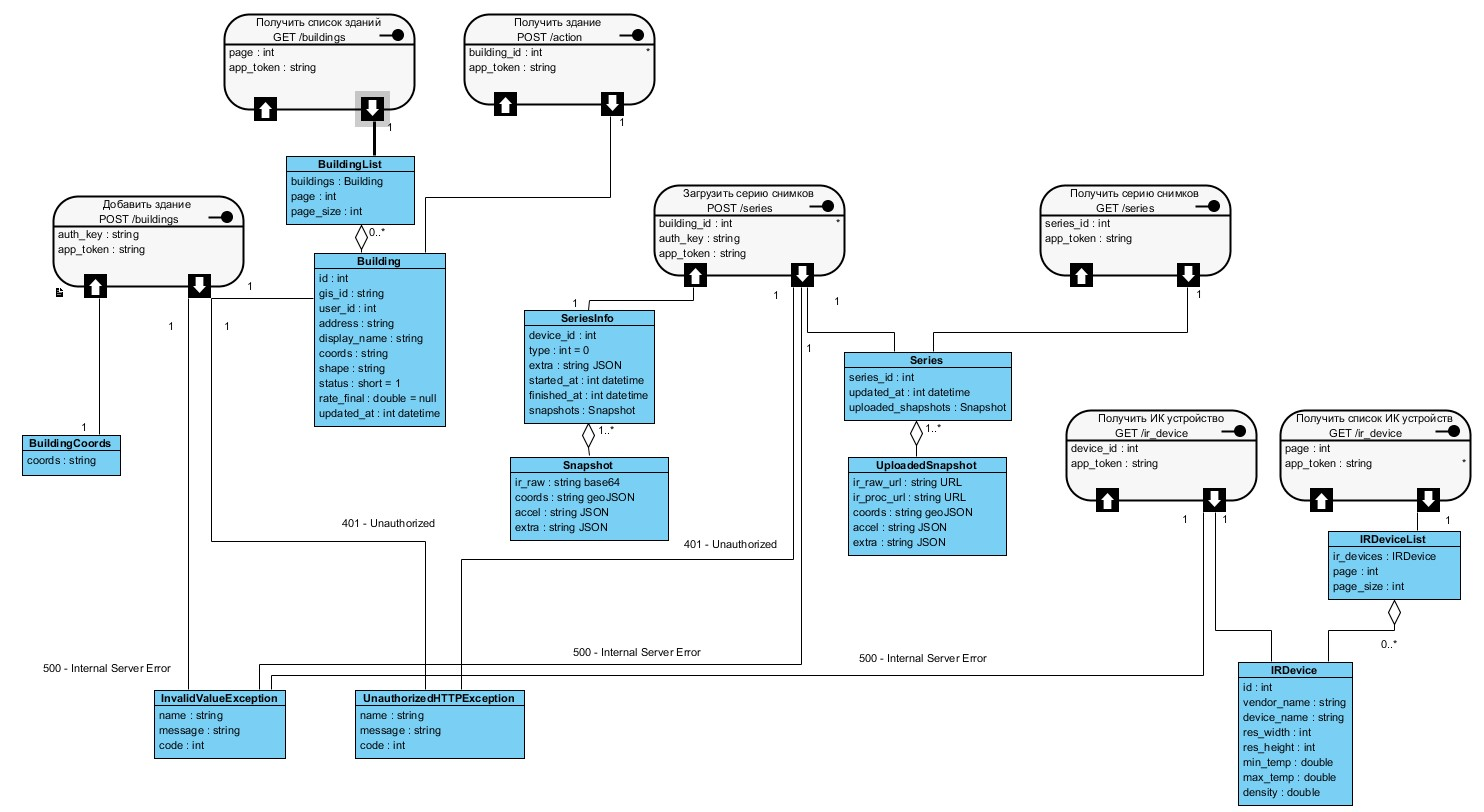
\includegraphics[width=1.3\textwidth]{images/uml/1}
		      \caption{Фрагмент диаграммы классов, описывающей структуру основной части API САТУ}
		      \label{uml:1}
		\end{figure}

	\end{landscape}

	\pagebreak

	Атрибуты некоторых классов в представленной диаграмме во многом совпадают с атрибутами сущностей в ER-диаграмме. Тем не менее, атрибуты классов показывают, что должен включать в себя тот или иной HTTP-запрос к ресурсу. При обращении к нему клиентская программа должна учитывать правильность соблюдения не только типов передаваемых данных, но и структуры отправляемого запроса.

	Некоторые классы связаны между собой отношением агрегации. Например, чтобы загрузить снимки какого-либо здания в систему, требуется передать данные о съёмке (класс \texttt{SeriesInfo}): идентификатор ИК устройства (\texttt{device\_id}), тип съёмки (\texttt{type}), а также несколько снимков (\texttt{snapshots}), где каждый снимок (класс \texttt{Snapshot}) описан четырьмя атрибутами: изображение, закодированное в формате base64, координаты снимка, данные встроенного акселерометра в формате JSON (\texttt{accel}) и т. п.

	В данной диаграмме обозначены классы \texttt{InvalidValueException}, \texttt{UnauthorizedHTTPException}, которые используются для оповещения клиентов об ошибках при передаче невалидных данных и при некорректной аутентификации/авторизации. HTTP-ответы, содержащие сведения об ошибке, API помечает соответствующим статусом. В соответствии с REST [ссылка], коды ошибок необходимо использовать по назначению, когда это возможно.

	\pagebreak

\section{Результаты и выводы по главе 3}

\par
	
	На основе полученных на этапе моделирования результатов сформулированы требования к разрабатываемому программному интерфейсу, определены программные средства и архитектурные принципы, которые легли в основу внутреннего проекта. Таким образом, были достигнуты следующие результаты:

	\begin{itemize}
		\item составлено Техническое задание на разработку системы (приложение \ref{app-tz});
		\item определён набор программных средств и инструментов для создания системы;
		\item разработаны решения по программной архитектуре системы.
	\end{itemize}
